\chapter{sXGP・4G/5Gの技術概要と標準化プロセスの課題}
\label{chap:background}

\section{sXGPと4G/5Gの概要}

\subsection{sXGPの位置づけ(免許不要・TD-LTE互換)}

sXGP(shared eXtended Global Platform)は、日本国内において免許不要帯である1.9GHz帯を使用するTD-LTE互換の通信規格である。2015年の電波法改正により、自営等BWAシステムとして制度化され、免許取得なしで基地局の設置・運用が可能となった。チャネル幅は10MHz、送信電力は基地局で1W以下、端末で200mW以下に制限されており、屋内利用を前提とした運用形態が想定されている。

sXGPの最大の特徴は、3GPP標準のLTE(特にTD-LTE)との互換性を維持しながら、免許不要で運用可能な点にある。これにより、一般的なLTE対応端末(スマートフォン等)がそのまま利用でき、研究・教育機関において実機を用いたモバイルネットワーク実験が法令遵守の範囲で実施可能となる。特に、電波暗室や特定実験試験局の許可を必要とする通常のLTE実験と比較して、導入の障壁が大幅に低減される。

一方で、sXGPには周波数帯域幅の制約(10MHz)やカバレッジの制限(屋内利用想定)といった限界も存在する。また、利用可能な基地局機器は限定的であり、研究用途では商用装置の転用やSDR(Software Defined Radio)を用いた実装が主流となる。本研究では、sXGPをeNBとして活用することで、4G RAN(UE・eNB)と5G Core(5GC)を接続する実機検証環境を構築し、実装ベース標準化を支援する検証基盤を提供する。

\subsection{4G RAN(UE・eNB)とEPC/5GCの要素}

4G LTEシステムは、UE(User Equipment)、eNB(evolved NodeB)、EPC(Evolved Packet Core)から構成される。UEとeNB間の無線インタフェースはUuインタフェースと呼ばれ、RRC(Radio Resource Control)プロトコルによって無線リソース管理が行われる。eNBとEPC間は、制御面(Control Plane)がS1-MMEインタフェース、ユーザ面(User Plane)がS1-Uインタフェースで接続される。

EPCの主要構成要素として、MME(Mobility Management Entity)、HSS(Home Subscriber Server)、SGWC/SGWU(Serving Gateway Control/User plane)、PGWC/PGWU(PDN Gateway Control/User plane)が存在する。MMEは加入者の認証・位置管理・セッション管理を担当し、S1-APプロトコルを用いてeNBと通信する。HSSは加入者情報データベースであり、認証鍵(K、OPc)やAMF値を管理する。SGWU/PGWUはGTP-U(GPRS Tunneling Protocol - User plane)トンネルを用いてユーザデータを転送する。

4G LTEにおける基本的な手順は、Attachプロシージャ(初期接続)、Authentication(認証)、Default Bearer確立、PDN接続確立から構成される。NAS(Non-Access Stratum)メッセージは、UEとMME間でエンドツーエンドに交換され、eNBは透過的に中継する。本研究では、4G RANからのS1-APメッセージを5GC向けのNGAPメッセージに変換するコンバータを実装することで、既存4G RAN資産を5GCと接続可能にする。

\subsection{5GCのアーキテクチャ(AMF/SMF/UPF等)}

5G Core(5GC)は、サービスベースアーキテクチャ(SBA: Service Based Architecture)を採用し、各ネットワーク機能(NF: Network Function)がHTTP/2ベースのサービスインタフェースを介して相互に通信する。主要なNFとして、AMF(Access and Mobility Management Function)、SMF(Session Management Function)、UPF(User Plane Function)、UDM(Unified Data Management)、AUSF(Authentication Server Function)、NRF(Network Repository Function)などが存在する。

AMFは、UEの登録管理・接続管理・モビリティ管理を担当し、NG-APプロトコルを用いてgNB(5G基地局)または本研究のs1n2-converterと通信する。SMFは、PDUセッション管理・QoS制御・UPF選択を担当し、AMFおよびUPFと連携してデータパスを確立する。UPFは、ユーザプレーンのトラフィック転送・QoS適用・課金情報収集を担当し、GTP-Uトンネルを終端する。

5GCにおける基本的な手順は、Registration(登録)、Authentication(認証)、PDU Session Establishment(セッション確立)から構成される。4G LTEと比較して、制御面とユーザ面の分離(CUPS: Control and User Plane Separation)が徹底されており、SMFとUPFの独立性が高い。また、NASメッセージは5G NAS形式となり、セキュリティコンテキストの導出方法も変更されている(KAMFからKNASint/KNASencを導出)。

本研究で利用する5GC機能範囲は、基本的な登録・認証・PDUセッション確立に限定し、ネットワークスライシング・エッジコンピューティング・ローカルブレイクアウトなどの高度な機能は対象外とする。実装にはOpen5GSを採用し、AMF、SMF、UPF、UDM、AUSF、NRF、PCF(Policy Control Function)などのNFをDockerコンテナとして展開する。

\section{3GPP標準化と標準-実装ギャップ}

\subsection{仕様の包含範囲とリファレンス実装の不足}

3GPP(3rd Generation Partnership Project)は、モバイル通信システムの標準化を行う国際的な組織であり、SA(Service and System Aspects)、CT(Core network and Terminals)、RAN(Radio Access Network)の3つの技術仕様グループ(TSG: Technical Specification Group)に分かれている。各TSGは複数のワーキンググループ(WG)を持ち、それぞれがTS(Technical Specification)やTR(Technical Report)を策定する。

例えば、5G Coreの基本アーキテクチャはTS 23.501、プロシージャはTS 23.502、NGAPはTS 38.413、5G NASはTS 24.501に規定されている。これらの仕様書は相互に参照関係を持ち、全体として数千ページに及ぶ膨大な文書群を形成している。仕様には必須(Mandatory)要件と任意(Optional)要件が混在し、実装者は必須要件のみを実装することが許容される。

しかし、3GPP仕様にはリファレンス実装が存在せず、仕様書の記述が実装レベルで曖昧な場合がある。例えば、エラー処理の詳細、タイマー値の推奨範囲、再送ポリシー、並行処理時の順序保証などは、仕様書に明示的に記載されていないことが多い。このため、ベンダ各社が独自に解釈・実装を行い、結果として実装間の相互運用性に課題が生じる。

研究においては、このような仕様の曖昧性が実験の再現性や比較可能性に影響を与える。特に、OSS実装(Open5GS、srsRAN等)は仕様の一部のみを実装しており、商用実装との機能差が存在する。本研究では、Open5GSを基盤として使用するが、実装上の制約を明示的に文書化し、検証範囲を明確にすることで、研究の内的妥当性を確保する。

\subsection{ベンダ実装差と相互接続性の課題}

モバイル通信システムの実装には、ベンダ固有の解釈や拡張が含まれることが一般的である。代表的なベンダ実装差として、以下が挙げられる:

\begin{itemize}
\item \textbf{Information Element(IE)の扱い}:任意IEの実装有無、未知IEの無視/拒否ポリシー、IE順序の依存性
\item \textbf{タイマー値とリトライ回数}:デフォルト値の差異、ネットワーク条件に応じた動的調整の有無
\item \textbf{再送とフォールバック}:メッセージ再送時の挙動、暗号化アルゴリズムのネゴシエーション失敗時の処理
\item \textbf{ベンダ拡張IE}:3GPP標準外の独自IEの追加、相互運用性試験での扱い
\end{itemize}

これらの実装差は、IOT(InterOperability Test)において顕在化する。特に、異なるベンダのUE/RAN/Coreを組み合わせた場合、標準仕様に準拠していても相互接続に失敗するケースが報告されている。既知の回避策として、IOTイベントでの事前検証、ベンダ間での実装ノートの共有、3GPP Change Request(CR)による仕様明確化などが行われている。

OSS実装においても、実装の成熟度や機能範囲の差が存在する。例えば、Open5GSはデータ通信機能を中心に実装されており、VoLTE/IMS、SMS over NAS、複数DNN選択などの機能は未実装または部分実装である。本研究では、基本的なデータ通信機能を中心に検証を行い、高度な機能については今後の拡張課題として位置づける。

\subsection{研究・評価におけるギャップの影響}

標準仕様と実装の乖離は、研究の再現性および比較可能性に重大な影響を与える。特に、以下の点が課題となる:

\begin{itemize}
\item \textbf{内的妥当性}:実験条件の統制が困難(実装依存の挙動、バージョン差異、設定パラメータの影響)
\item \textbf{外的妥当性}:OSS実装での検証結果が商用環境に適用可能か不明(機能範囲の差、性能特性の違い)
\item \textbf{再現性}:実装のバージョン、設定ファイル、依存ライブラリのバージョンが論文に明記されないことが多い
\end{itemize}

これらの課題に対する対策として、本研究ではOSS実装を用いた検証基盤の構築を提案する。具体的には、Docker化による環境の固定化、設定ファイルやスクリプトの公開、パケットキャプチャの保存により、第三者による検証の再現を可能にする。また、実装の制約を明示的に文書化することで、検証結果の適用範囲を明確にする。

さらに、IETFの"rough consensus and running code"原則に倣い、実装を動かしながら標準化にフィードバックするアプローチを採用する。これにより、仕様の曖昧性や実装上の問題点を早期に発見し、標準化サイクルの短縮に貢献することを目指す。

\section{RAN–コア間インターワーキングの基礎}

\subsection{制御面(S1-AP vs. NG-AP)}

4G LTEにおけるeNBとMME間の制御面プロトコルはS1-AP(S1 Application Protocol)であり、5GにおけるgNBとAMF間の制御面プロトコルはNG-AP(NG Application Protocol)である。両プロトコルはASN.1(Abstract Syntax Notation One)で定義され、SCTP(Stream Control Transmission Protocol)上で動作する点は共通であるが、メッセージ構造やInformation Element(IE)の定義が異なる。

表\ref{tab:s1ap_ngap_mapping}に、主要なS1-APとNG-APメッセージの対応関係を示す。

\begin{table}[htbp]
\centering
\caption{S1-APとNG-APの主要メッセージ対応}
\label{tab:s1ap_ngap_mapping}
\begin{tabular}{|l|l|l|}
\hline
\textbf{手順} & \textbf{S1-AP} & \textbf{NG-AP} \\
\hline
初期接続 & InitialUEMessage & InitialUEMessage \\
\hline
初期コンテキスト設定 & InitialContextSetupRequest & InitialContextSetupRequest \\
\hline
初期コンテキスト設定応答 & InitialContextSetupResponse & InitialContextSetupResponse \\
\hline
NAS下り転送 & DownlinkNASTransport & DownlinkNASTransport \\
\hline
NAS上り転送 & UplinkNASTransport & UplinkNASTransport \\
\hline
UEコンテキスト解放要求 & UEContextReleaseRequest & UEContextReleaseRequest \\
\hline
\end{tabular}
\end{table}

メッセージ名は類似しているが、含まれるIEの内容は大きく異なる。特に、セッション管理に関連するIEは、4GのBearer概念から5GのPDU Session概念への変更に伴い、大幅に再設計されている。例えば、4GのE-RAB(E-UTRAN Radio Access Bearer)は5GのPDU Session Resourceに対応するが、QoS制御の粒度が異なる(4GはBearer単位、5GはQoS Flow単位)。

本研究で実装するs1n2-converterは、S1-APメッセージを受信してNG-APメッセージに変換する。変換時の主要なポイントとして、以下が挙げられる:

\begin{itemize}
\item UE識別子の変換(MME-UE-S1AP-ID ↔ AMF-UE-NGAP-ID、eNB-UE-S1AP-ID ↔ RAN-UE-NGAP-ID)
\item E-RAB情報からPDU Session情報への変換(E-RAB ID → PDU Session ID、QCI → 5QI)
\item GTP-Uトンネル情報の抽出と再マッピング(TEID、Transport Layer Address)
\item NASメッセージのカプセル化(4G NAS → 5G NAS変換は別途実施)
\end{itemize}

エラー処理については、変換不可能なIEが含まれる場合や、必須IEが欠落している場合の処理方針を定義する必要がある。本研究では、基本的なデータ通信に必要なIEのみを変換し、未対応のIEについてはログに記録した上でスキップする方針を採用する。

\subsection{ユーザ面(GTP-U互換性とパススルー/変換)}

ユーザ面プロトコルであるGTP-U(GPRS Tunneling Protocol - User plane)は、4Gと5Gで基本的に互換性が維持されている。GTP-Uは、IPパケットをカプセル化してトンネル転送するプロトコルであり、TEID(Tunnel Endpoint Identifier)を用いて各トンネルを識別する。

GTP-Uトンネルの確立は、制御面メッセージ(S1-AP/NG-AP)によって指示される。4Gでは、InitialContextSetupRequestメッセージにE-RAB Setup ListとしてTEIDとTransport Layer Address(IPアドレス)が含まれる。5Gでは、PDUSessionResourceSetupRequestメッセージにPDU Session Resource Setup Request Transferとして同様の情報が含まれる。

本研究で実装するs1n2-converterは、GTP-Uパケットの中継を行う。具体的には、以下の処理を実施する:

\begin{itemize}
\item \textbf{S1-U → N3方向}:4G eNBからのGTP-Uパケットを受信し、TEID変換テーブルを参照して5G UPF向けのTEIDに書き換え、N3インタフェース(5G UPF)に転送
\item \textbf{N3 → S1-U方向}:5G UPFからのGTP-Uパケットを受信し、TEID変換テーブルを参照して4G eNB向けのTEIDに書き換え、S1-Uインタフェース(4G eNB)に転送
\end{itemize}

TEID割り当てについては、s1n2-converter自身が上り方向と下り方向のTEIDを独立に管理し、eNB側とUPF側に対してそれぞれ異なるTEIDを割り当てる。これにより、eNBとUPFが同じTEID空間を共有する必要がなくなり、TEID衝突のリスクを回避できる。

QoS制御については、4GのQCI(QoS Class Identifier)と5Gの5QI(5G QoS Identifier)の対応関係を定義し、変換を行う。標準化されたQCI/5QIの対応関係は3GPP TS 23.501に規定されているが、本研究では基本的なデータ通信(QCI=9 → 5QI=9)のみを対象とする。

MTU(Maximum Transmission Unit)とフラグメント処理については、GTP-Uヘッダのオーバーヘッド(8バイト + UDPヘッダ8バイト + IPヘッダ20バイト = 36バイト)を考慮し、必要に応じてPath MTU Discoveryを実施する。ただし、本研究の実験環境はDocker内部ネットワークを使用するため、MTU問題は発生しにくい。

\subsection{ID/コンテキスト管理(NAS, IMSI/SUPI 等)}

モバイルネットワークにおけるUE識別子は、永続的識別子と一時的識別子に分類される。4Gでは、永続的識別子としてIMSI(International Mobile Subscriber Identity)、一時的識別子としてGUTI(Globally Unique Temporary Identifier)が使用される。5Gでは、永続的識別子としてSUPI(Subscription Permanent Identifier)、一時的識別子として5G-GUTIが使用される。

IMSI/SUPIの形式は類似しており、MCC(Mobile Country Code)、MNC(Mobile Network Code)、MSIN(Mobile Subscription Identification Number)から構成される。本研究では、4GのIMSIを5GのSUPIとして扱い、識別子の変換を行わない方針を採用する。これは、Open5GS HSSとUDMが同一の加入者データベース(MongoDB)を共有しており、IMSIベースでの管理が可能なためである。

NASセキュリティコンテキストは、UEとMME/AMF間のNASメッセージを保護するために使用される。4Gでは、認証成功後にKASME(Key Access Security Management Entity)が導出され、そこからKNASint(NAS Integrity Key)とKNASenc(NAS Encryption Key)が導出される。5Gでは、認証成功後にKAMF(Key Access and Mobility Management Function)が導出され、そこからKNASint/KNASencが導出される。

鍵導出のアルゴリズムは4Gと5Gで異なり、単純な変換は不可能である。本研究では、s1n2-converterがNASメッセージの変換を行う際に、NAS Integrity Protectionの検証を行わない方針を採用する。これは、4G eNBと5G AMF間でNASセキュリティコンテキストが共有されないためである。ただし、この方針はセキュリティ上のリスクを伴うため、実験環境に限定した運用とし、本番環境での使用は推奨しない。

コンバータ内でのUEコンテキスト管理については、S1-AP UE IDとNG-AP UE IDのマッピングテーブルを維持し、メッセージ変換時に参照する。また、GTP-U TEIDマッピングテーブルも同様に維持し、ユーザ面パケットの中継時に使用する。これらのテーブルは、UEContextReleaseRequestメッセージ受信時にクリーンアップされる。

\section{OSSと6Gに向けた開発・検証サイクル}

\subsection{OSSの役割(Open5GS等)と試作の加速}

Open Source Software(OSS)は、モバイルネットワーク研究における重要な基盤となっている。特に、Open5GSは4G EPC/5G Coreの包括的な実装を提供し、世界中の研究機関や企業で広く利用されている。Open5GSの主な特徴として、以下が挙げられる:

\begin{itemize}
\item \textbf{モジュール構成}:各ネットワーク機能(MME、AMF、SMF、UPF等)が独立したプロセスとして実装され、マイクロサービスアーキテクチャを採用
\item \textbf{拡張性}:C言語で実装され、ソースコードが公開されているため、独自機能の追加や動作のカスタマイズが容易
\item \textbf{活発なコミュニティ}:GitHub上で継続的に開発が行われており、バグ修正や新機能追加が頻繁にリリースされる
\item \textbf{標準準拠}:3GPP仕様に基づいた実装が行われており、商用実装との相互運用性が考慮されている
\end{itemize}

OSSを活用することで、研究プロトタイプの実装速度が大幅に向上する。商用装置を用いた実験では、ベンダとの契約や機器調達に数ヶ月を要するのに対し、OSSを用いた実験環境は数日で構築可能である。また、学習コストも低減される。Open5GSはドキュメントが充実しており、Webベースの管理画面(WebUI)を提供するため、初学者でも容易に環境構築が可能である。

本研究では、Open5GSを基盤として使用し、4G EPCおよび5G Coreを構築する。さらに、srsRAN(旧srsLTE)をRANシミュレータとして使用し、ZMQ(ZeroMQ)ベースのRF simulationによってeNB/gNBとUEを接続する。これにより、物理的な無線機器を必要とせず、ソフトウェアのみで完全なEnd-to-End環境を構築できる。

\subsection{適合・相互接続・回帰テストの自動化}

モバイルネットワークの品質保証には、適合性試験(Conformance Test)、相互運用性試験(InterOperability Test)、回帰試験(Regression Test)が不可欠である。これらの試験を手動で実施することは時間とコストがかかるため、自動化の仕組みが重要となる。

自動試験の枠組みとして、以下のアプローチが考えられる:

\begin{itemize}
\item \textbf{シナリオ駆動試験}:試験シナリオをスクリプトまたはYAML/JSON形式で記述し、試験フレームワークが自動的に実行
\item \textbf{パケットキャプチャ照合}:Wireshark/tsharkを用いてパケットキャプチャを取得し、期待されるメッセージシーケンスと照合
\item \textbf{ログ解析}:各ネットワーク機能のログ出力を解析し、エラーメッセージや警告の有無を検証
\item \textbf{差分検出}:基準となる「正常動作時」のパケットキャプチャ/ログと、変更後の結果を比較し、差分を自動検出
\end{itemize}

既存のテスト資産として、TTCN-3(Testing and Test Control Notation version 3)を用いた適合性試験ツールが存在する。TTCN-3は、通信プロトコルのテストケースを形式的に記述するための言語であり、3GPP標準化においても参照されている。ただし、TTCN-3の学習コストは高く、研究用途では軽量なスクリプトベースのアプローチが好まれる。

本研究では、基本的なEnd-to-End接続性を確認するための最小限の回帰テストセットを設計する。具体的には、以下のシナリオを自動実行し、成功/失敗を判定する:

\begin{enumerate}
\item 4G Attach + Default Bearer確立 + Ping疎通
\item 5G Registration + PDU Session確立 + Ping疎通
\item 4G → 5G変換環境でのAttach + Session確立 + Ping疎通
\end{enumerate}

これらのテストは、Docker Composeを用いた環境起動スクリプトと組み合わせることで、完全に自動化可能である。将来的には、CI/CD(Continuous Integration / Continuous Deployment)パイプラインに統合し、コード変更のたびに自動的に実行することを想定している。

\subsection{再現性(Docker等)と研究公開の促進}

研究の再現性を確保するためには、実験環境の詳細な記録と共有が不可欠である。しかし、モバイルネットワーク実験は多数のコンポーネント(UE、RAN、Core)と複雑な設定を伴うため、環境再現が困難であることが多い。

Dockerコンテナ技術を活用することで、この課題を大幅に軽減できる。Dockerは、アプリケーションとその依存関係を単一のコンテナイメージとしてパッケージ化し、異なる環境で同一の動作を保証する技術である。本研究では、以下の方針でDocker化を実施する:

\begin{itemize}
\item \textbf{固定バージョン}:Open5GS、srsRAN、依存ライブラリのバージョンをDockerfileに明示的に記述
\item \textbf{設定ファイル共有}:各ネットワーク機能の設定ファイル(YAML形式)をGitリポジトリで管理
\item \textbf{ネットワーク構成の明示}:Docker Composeを用いて、コンテナ間のネットワーク構成(IPアドレス、サブネット、ブリッジ)を定義
\item \textbf{ログとパケットキャプチャの保存}:実験結果として、各コンポーネントのログファイルとWiresharkパケットキャプチャを保存
\end{itemize}

研究成果を公開する際には、以下の留意点がある:

\begin{itemize}
\item \textbf{認証鍵の除去}:HSS/UDMに登録された加入者の認証鍵(K、OPc)はダミー値に置き換える
\item \textbf{個人情報の除去}:IMSI、MSISDN、IPアドレスなどの個人情報は匿名化またはダミー値に置き換える
\item \textbf{ライセンス確認}:使用したOSSのライセンス(Apache、GPL等)を確認し、派生物の公開条件を遵守
\end{itemize}

本研究では、GitHub上でソースコード、設定ファイル、実験手順書を公開することを計画している。これにより、第三者が同一の実験環境を再現し、検証結果を確認できるようにする。また、Docker Hubにコンテナイメージを公開することで、環境構築の手間をさらに削減することも検討している。

\section{モバイルシステム全体での課題感}

\subsection{研究環境のコストとライセンス(免許・機器費用)}

モバイルネットワーク研究における最大の障壁の一つは、実機環境構築のコストと法的手続きである。典型的な4G/5G研究環境を構築する場合、以下の費用が発生する:

\begin{itemize}
\item \textbf{端末/モデム}:LTE/5G対応スマートフォンまたはUSBモデムで、数万円〜数十万円(研究用途では複数台必要)
\item \textbf{基地局(eNB/gNB)}:商用装置は数百万円〜数千万円、研究用小型基地局でも数十万円〜数百万円
\item \textbf{SDR(Software Defined Radio)}:USRP B210(約50万円)、LimeSDR(約5万円)など
\item \textbf{アンテナ・RF機器}:周波数帯に応じた適切なアンテナ、増幅器、フィルタなど
\item \textbf{測定機器}:スペクトラムアナライザ、シグナルジェネレータ、ネットワークアナライザなど(数百万円〜)
\end{itemize}

さらに、電波法に基づく免許取得または特定実験試験局の申請が必要となる。申請には技術基準適合証明(技適)の有無、使用周波数帯、出力電力、設置場所の詳細な情報が求められ、承認までに数週間〜数ヶ月を要する。また、屋外での実験は原則として禁止されており、電波暗室の使用が推奨されるが、電波暗室の建設・維持コストも高額である。

sXGP採用によるコスト/手続き削減効果は顕著である。sXGPは免許不要帯を使用するため、免許申請が不要であり、屋内であれば比較的自由に実験が可能である。基地局機器としては、LimeSDRなどの低コストSDRを用いることで、数万円程度で環境構築が可能となる。本研究では、ZMQベースのRF simulationを使用することで、さらにコストを削減し、ソフトウェアのみで完全な実験環境を構築している。

\subsection{相互接続性・ベンダ依存の壁}

モバイルネットワーク実験における相互接続性の課題は、複数のレイヤーで発生する:

\begin{itemize}
\item \textbf{UE/モデム差}:チップセットベンダ(Qualcomm、MediaTek、Exynos等)による実装差、OSバージョン(Android、iOS)の影響
\item \textbf{カーネル/ドライバ差}:LinuxカーネルのNetfilter/iptables設定、NICドライバのTCO(TCP Checksum Offload)やGRO(Generic Receive Offload)の挙動
\item \textbf{RAN実装差}:商用基地局、研究用小型基地局、SDRベース実装の機能範囲とタイミング精度の違い
\item \textbf{Core実装差}:Open5GS、商用EPC/5GC、他のOSS実装(free5GC、OAI等)の機能カバレッジと相互運用性
\end{itemize}

これらの差異は、実験結果の再現性と汎用性に影響を与える。例えば、特定のUEでは成功する手順が、別のUEでは失敗するケースが報告されている。また、Linux環境でのパケット転送性能は、NICオフロード機能の有効/無効によって大きく変動する。

評価設計での緩和策として、以下のアプローチが考えられる:

\begin{itemize}
\item \textbf{多様な端末での検証}:複数のベンダ/OSの端末を用いて、実装依存性を明らかにする
\item \textbf{OSS実装の組み合わせ}:Open5GS、free5GC、srsRANなど、複数のOSS実装を試験することで、標準準拠度を評価
\item \textbf{設定の明示的な文書化}:カーネルバージョン、NIC設定、オフロード機能の有効/無効を明記
\end{itemize}

本研究では、Open5GSとsrsRANの組み合わせを基本構成とし、実装の制約を明示的に文書化する。将来的には、他のOSS実装との相互運用性試験を実施することを計画している。

\subsection{運用・再現性とオープンテストベッドの不足}

モバイルネットワーク研究において、共有可能なテストベッドの不足は長年の課題である。研究機関ごとに独自の環境を構築しているが、環境の詳細が論文に記載されないことが多く、第三者による再現が困難である。また、商用ネットワークを用いた実験は、ベンダとの契約やセキュリティ上の制約から、詳細な実験条件を公開できないことが多い。

オープンテストベッドの事例として、米国のPOWDER(Platform for Open Wireless Data-driven Experimental Research)やヨーロッパのONELab(Open Network Laboratory)が存在する。これらは、研究者が遠隔からアクセス可能なテストベッドを提供し、実機を用いた実験を支援している。しかし、利用にはアカウント登録や審査が必要であり、自由度が制限される場合がある。

本研究では、Docker化された実験環境を提供することで、第三者が自身の環境で実験を再現できるようにする。提供するアーティファクトとして、以下を計画している:

\begin{itemize}
\item \textbf{Dockerコンテナイメージ}:Open5GS、srsRAN、s1n2-converterを含む完全なシステム
\item \textbf{設定ファイル}:各コンポーネントのYAML設定ファイル、ネットワーク構成
\item \textbf{実験スクリプト}:環境起動、UE接続、データ通信確認、ログ収集の自動化スクリプト
\item \textbf{パケットキャプチャ}:Wiresharkで解析可能なpcapファイル(S1-AP、NG-AP、GTP-U、NAS)
\item \textbf{実験手順書}:セットアップから実験実施、結果確認までの詳細な手順
\end{itemize}

これにより、研究成果の再現性を確保し、他の研究者が本研究を基盤として発展させることを可能にする。

\subsection{セキュリティ・計測基盤の一般化の難しさ}

モバイルネットワーク実験におけるセキュリティ上の課題は、以下の通りである:

\begin{itemize}
\item \textbf{認証鍵の取り扱い}:HSS/UDMに登録された加入者の認証鍵(K、OPc)は、SIMカード内に格納されており、外部からの読み取りは困難。実験用途では、ダミー鍵を使用するか、eUICC(embedded Universal Integrated Circuit Card)を用いたプログラマブルSIMを使用する必要がある
\item \textbf{プライバシ/PII(Personally Identifiable Information)}:IMSI、MSISDN、位置情報などの個人識別可能な情報は、研究成果公開時に匿名化またはダミー値に置き換える必要がある
\item \textbf{攻撃面の考慮}:実験環境が外部ネットワークに接続されている場合、セキュリティホール(例:認証バイパス、暗号化無効化)が攻撃経路となるリスクがある
\item \textbf{計測オーバーヘッド}:パケットキャプチャ、ログ記録、性能計測ツールの実行によるCPU/メモリオーバーヘッドが、実験結果に影響を与える可能性がある
\end{itemize}

本研究では、実験環境を外部ネットワークから隔離されたDockerネットワーク内に構築することで、セキュリティリスクを最小化する。また、認証鍵やIMSIはダミー値を使用し、研究成果公開時には個人情報を含まないように配慮する。計測オーバーヘッドについては、本格的な性能評価を行う際には計測ツールの影響を定量化し、補正を行う方針とする。

\section{法規制とsXGPの位置づけ}

\subsection{電波法の制約と実機検証の困難}

日本国内における無線通信実験は、電波法によって厳格に規制されている。主な制約として、以下が挙げられる:

\begin{itemize}
\item \textbf{屋内外の制約}:屋外での電波発射には原則として無線局免許が必要。屋内実験でも、電波漏洩を防ぐための電波暗室の使用が推奨される
\item \textbf{出力制限}:免許不要帯以外の周波数帯を使用する場合、特定実験試験局として申請が必要。出力電力は用途に応じて制限される
\item \textbf{使用帯域}:LTE Band 1(2.1GHz)、Band 3(1.8GHz)、5G n77(3.7GHz)、n79(4.5GHz)などの商用周波数帯は、免許取得または実験試験局申請が必須
\item \textbf{干渉リスク}:実験電波が商用ネットワークや他の無線システムに干渉を与えるリスクがあり、周波数調整や出力制限が求められる
\end{itemize}

学術機関での典型的な許認可フローは、以下の通りである:

\begin{enumerate}
\item 実験計画書の作成(使用周波数、出力電力、実験期間、設置場所の詳細)
\item 技術基準適合証明(技適)の確認、またはシールドルーム使用計画
\item 総務省総合通信局への特定実験試験局の申請
\item 審査期間(通常2週間〜1ヶ月)
\item 免許交付後、実験開始
\item 実験終了後、結果報告書の提出
\end{enumerate}

このプロセスは、迅速なプロトタイピングや反復実験を前提とする研究開発には不向きである。特に、学生や若手研究者が短期間で実験環境を構築し、試行錯誤を繰り返すことが困難となる。

\subsection{免許不要帯を用いた代替アプローチとしてのsXGPの意義}

sXGPは、免許不要帯(1.9GHz帯)を使用することで、上記の法的制約を大幅に緩和する。sXGPの法的位置づけは、電波法施行規則第6条第4項第3号の6に規定される「小電力データ通信システムの無線局」に該当し、技術基準適合証明(技適)を取得した機器であれば、免許取得なしで運用可能である。

sXGPを用いた実機検証の意義は、以下の通りである:

\begin{itemize}
\item \textbf{法令遵守}:免許申請不要で、合法的に実機相当のRAN実験が可能
\item \textbf{迅速な環境構築}:機器の調達から実験開始までの期間が大幅に短縮(数日〜数週間)
\item \textbf{反復実験の容易化}:設定変更や機能追加を繰り返し、試行錯誤が可能
\item \textbf{教育利用}:学生が自主的にモバイルネットワーク実験を行える環境を提供
\end{itemize}

一方で、sXGPには以下の限界も存在する:

\begin{itemize}
\item \textbf{周波数帯域幅}:10MHzに制限されており、高スループット実験(例:100Mbps以上)には不向き
\item \textbf{設備可用性}:sXGP対応基地局機器は限定的であり、商用装置の入手は困難。研究用途ではSDRを用いた自作が主流
\item \textbf{カバレッジ}:送信電力が制限されており(基地局1W、端末200mW)、広範囲のカバレッジ実験には不向き
\item \textbf{商用環境との差異}:商用LTE/5Gネットワークとは周波数帯・出力・設定が異なるため、結果の外的妥当性に留意が必要
\end{itemize}

本研究では、sXGPの利点を活かしつつ、限界を認識した上で実験設計を行う。特に、基本的なプロトコル変換機能と相互運用性の検証に焦点を当て、高スループットや広域カバレッジは今後の課題として位置づける。sXGPを用いることで、実装ベース標準化を支援する検証基盤を低コストかつ法令遵守の範囲で提供し、モバイルネットワーク研究の民主化に貢献することを目指す。

\section{シミュレータの対象範囲と限界}
\subsection{シミュレーションで十分な領域}
新NFのアルゴリズム検討、プロトコル状態機械の基本遷移の正当性確認、ラフなスケール試験、CIでの高速回帰などはシミュレータで効率的に実施できる。
\subsection{シミュレーションの限界}
実UE固有の実装差(RRC/NASのタイマ・再送・Capability差)、RRC/PHY/MACの時間ゆらぎ由来の境界条件、OS/NICのオフロードやキューイング、パケット順序入替・フラグメンテーション、S1AP$\leftrightarrow$NGAP変換やTEID管理の例外パスなどは、シミュレータでは再現が難しい。

\section{実機が必要となる検証項目}
\begin{itemize}
	\item 厳密なタイマ境界・再送・例外遷移(登録/PDU確立、NAS/RRCの異常系)
	\item セキュリティと鍵管理(AKA/EAP-AKA'、KDF、再同期、アルゴ協定の実装差)
	\item ユーザ面の実性能(GTP-Uオフロード、カーネル/DPDK、NUMA/CPUスケジューリング)
	\item 相互接続・回帰(複数UE/モデム/OSでの互換性検証)
	\item フェイルシナリオ(部分ロス、遅延、再順序化、NICドロップ、CPUスタベーション)
\end{itemize}

\section{本環境がもたらす価値(ユースケース)}
\label{sec:values}
\subsection{教育・トレーニング}
免許不要帯で運用可能なsXGPをeNBとして活用し、4G RANと5GCを接続できるため、学部・大学院・企業研修において、法令遵守のもとで実機に近い無線・コア連携の学習が可能となる。設定の再現手順を公開することで、実験レポートの客観性と再現性も高められる。

\subsection{プロトタイピングと検証の高速化}
コントロールプレーン(S1AP/NGAP/NAS)およびユーザプレーン(GTP-U)の変換・中継部を差し替え可能にすることで、新しいアルゴリズムやポリシー(例:識別子管理、TEID割当、タイムアウト制御)の試作・検証を低コストで繰り返し実施できる。

\subsection{相互接続・回帰テスト}
Open5GSなどの5GC実装や各種eNB/UEに対して、信令互換性や基本機能(登録、PDUセッション確立)の回帰テストを自動化できる。コンバータを介した差分吸収により、ベンダ差や仕様差を可視化しつつ評価できる。

\subsection{性能評価とボトルネック分析}
遅延・スループット・リソース使用率(CPU/メモリ)の計測基盤を同梱することで、コンバータの処理遅延やカプセル化オーバヘッド、TEID管理戦略の影響を定量化でき、設計改善に資する。

\subsection{再現性の高い研究公開と共同研究}
Dockerを用いた構成管理とビルド手順の統一により、第三者が同一環境で追試できる。研究成果の普及や共同研究の立ち上げコストを下げる。

\subsection{運用研究・障害シナリオの再現}
認証失敗やセキュリティモードエラー、ハンドオーバ相当の遷移など、現場で発生しうる事象の再現とトラブルシュート手順の確立に役立つ。

\section{本研究が対象とする課題の定義}
\subsection{研究者・学生が手軽に再現できる環境の要件}
必要構成要素・費用・所要時間・依存関係・再現手順の粒度を定義し、到達すべきユーザ体験(セットアップから成功確認まで)を示す。
\subsection{sXGP×5GC接続の技術的論点の範囲}
本研究で扱う範囲(制御/ユーザ面の変換、識別子/セキュリティ/状態管理)と扱わない範囲(RRC/PHY最適化、商用品質の最適化など)を明確化する。
\subsection{評価指標と成功基準の設定}
機能(登録/セッション確立率)、性能(遅延/スループット/CPU等)、堅牢性(異常時の復帰)、再現性(環境差耐性)の指標と合格基準を定める。


% (注)宇宙通信に関する章は本研究スコープ外のため削除。

% (注)該当節を削除。


% (注)該当節を削除。


% (注)該当節を削除。

% (注)DTN記述は別研究のため削除。

% \subsection{通信機会の非対称性}
% \label{subsection:通信機会の非対称性}

% \begin{figure}[tbh]
%     \centering
%     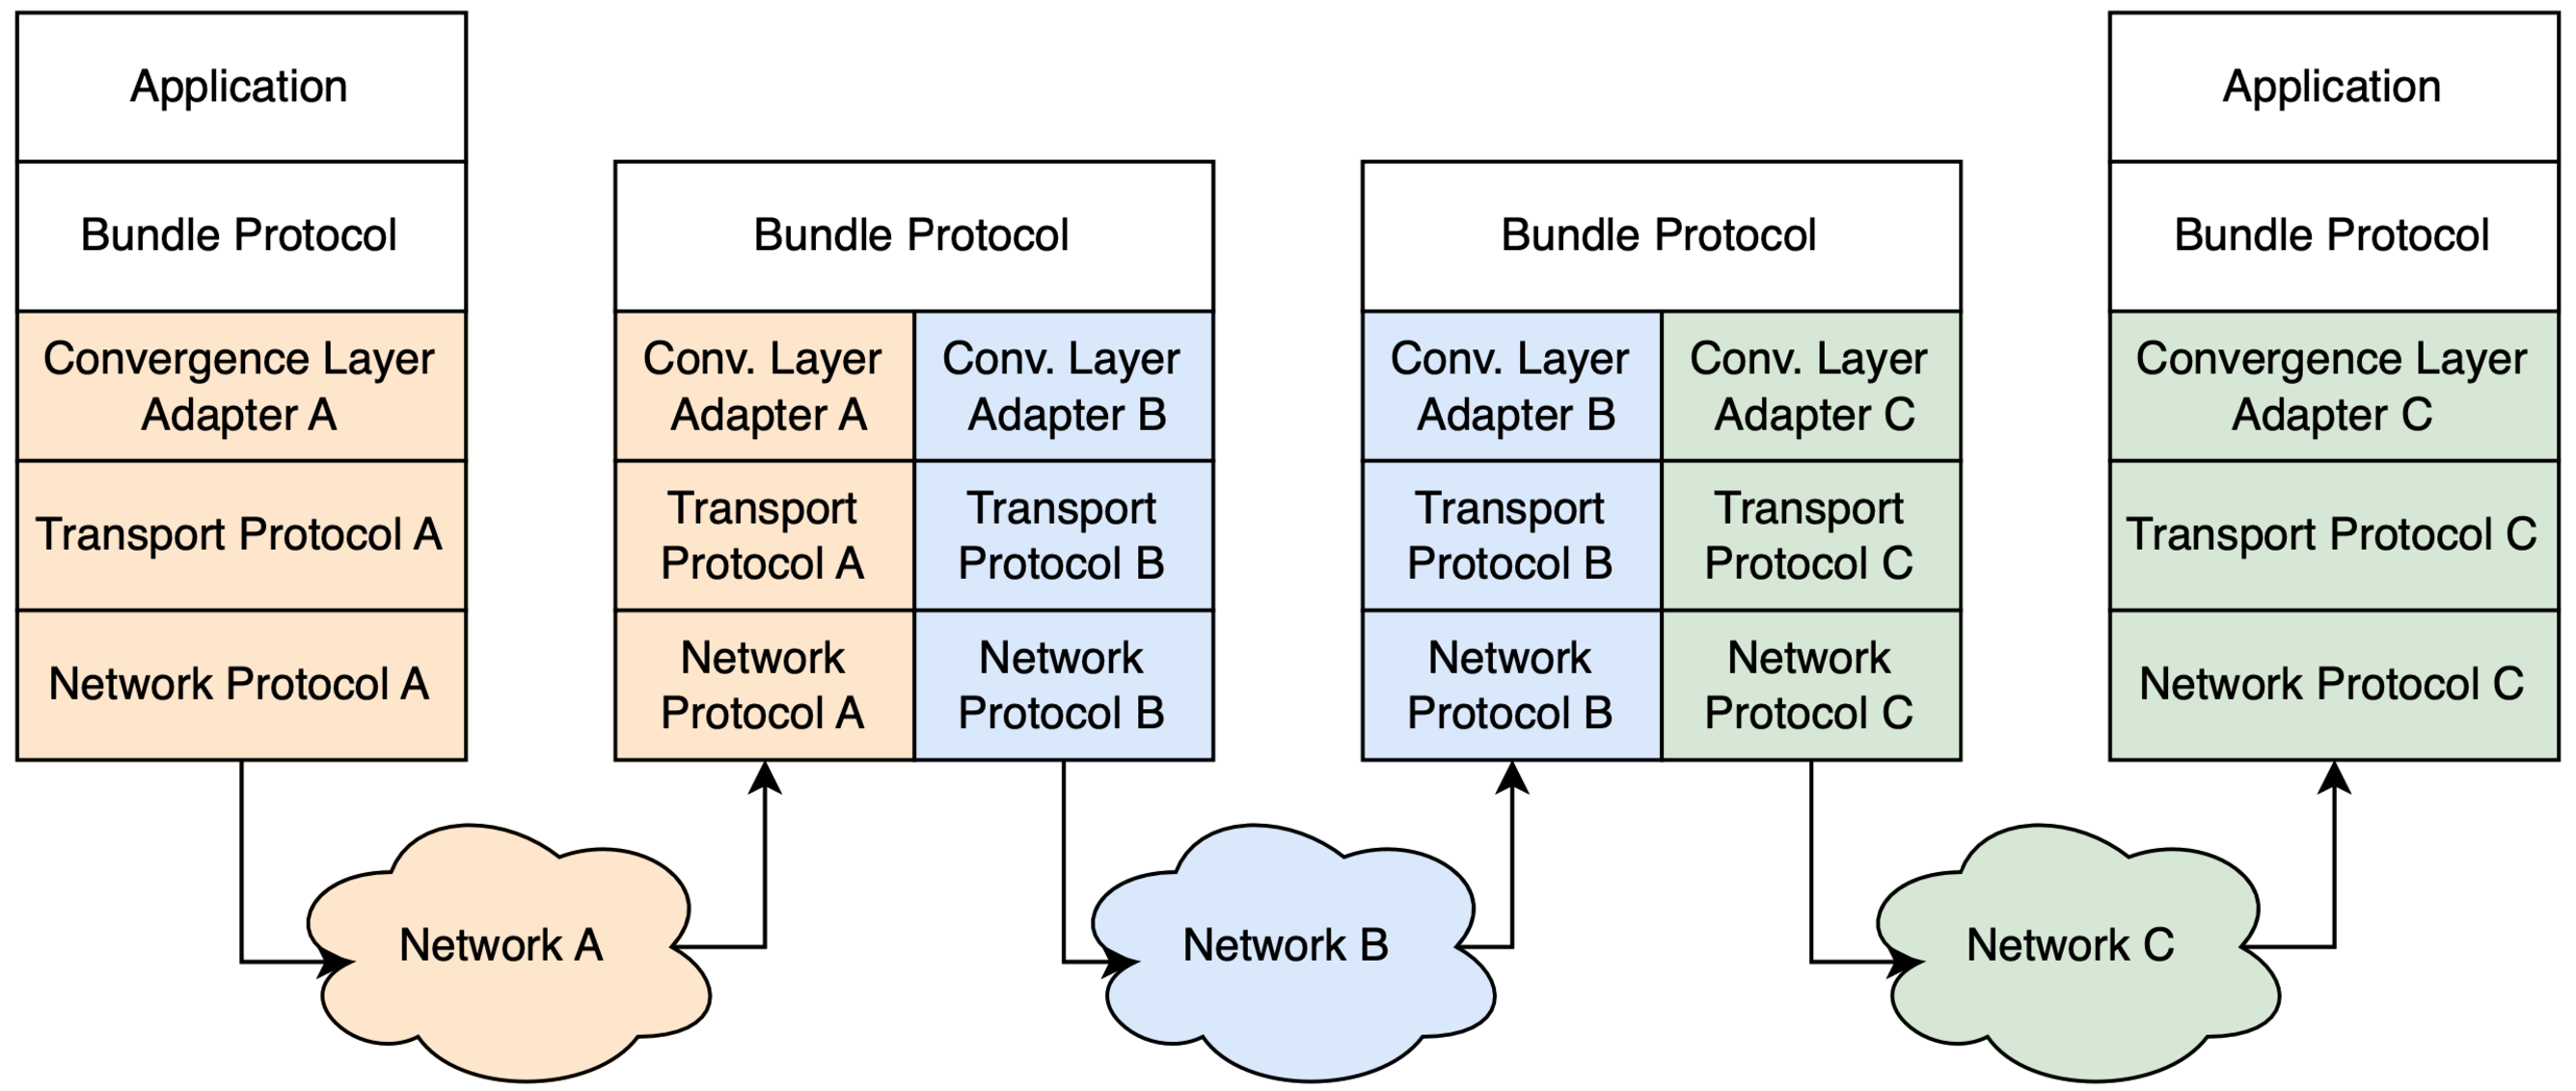
\includegraphics[width=0.7\textheight]{img/dtnprotocolstack.pdf}
%     \caption{DTNを搭載したノード間のみでの通信}
%     \label{fig:dtnprotocolstack}
%     \begin{minipage}{\textwidth}
%         \raggedright
%         \vspace{3mm}
%         \fontsize{10.5pt}{12pt}\selectfont
%         参考文献\cite{bundle_protocol_architecture}Figure1をもとに作成.
%         図中のConvergence Layer(CL)については
%         \ref{section:Convergence LayerとLTP}項で説明する.
%     \end{minipage}
% \end{figure}

% (注)該当節を削除。

% (注)該当節を削除。

% (注)該当節を削除。

% (注)該当節を削除。

% (注)該当節を削除。

% \begin{table}[tbh]
%     \centering
%     \caption{DTN実装とその機能の比較}
%     \begin{minipage}[t]{\textwidth}
%         \centering
%         \fontsize{10.5pt}{12pt}\selectfont
%         参考文献\cite{dtn_implementations}figure1より抜粋
%         \vspace{3mm}
%     \end{minipage}
%     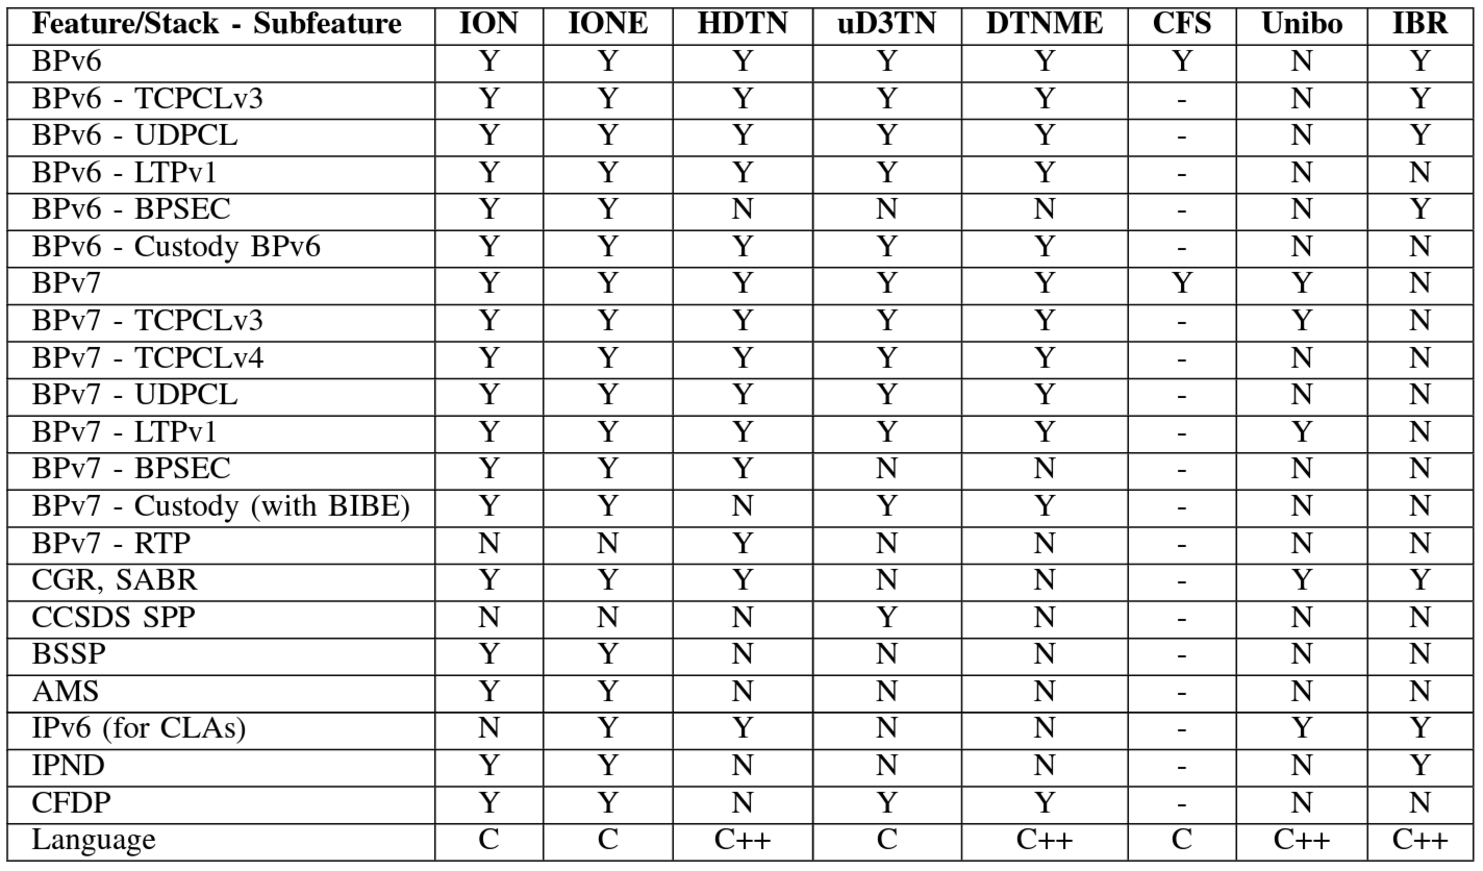
\includegraphics[width=0.7\textheight]{img/chart_dtn_implementations.pdf}
%     \label{table:chart_dtn_implementations}
% \end{table}
